\chapter{Installation}
\label{cha:Installation}
\section{How to Build \CGG{} from Developer's Git Repository}%
\label{sec:How_to_build}

These are generic build instructions for building \CGG{} Infinity.  
Known to work on Ubuntu, Mint, OpenSuse, Fedora, Debian, Centos, Arch, Slackware, and Gentoo. 
It has not been tested on every single possible distro yet so you might expect to have to make some minor changes.
Also works on a somewhat limited basis on FreeBSD and Windows 10 with the bsd.patch for FreeBSD
and the cygwin.patch for Windows 10.

Alternatively, there are some pre-built dynamic or static binaries which are updated on a fairly regular basis (as long as code changes have been made) available at the link below.

\begin{center}
	{\small \url{https://cinelerra-gg.org/download/}}
\end{center}

There are 2 kinds of builds, the default system-build and a single-user build.  
A system build has results which are installed to the system. 
The majority of the files are installed in the standard system paths, but some customization is possible. 
The single user build allows for running completely out of a local user directory so it doesn't affect the system.

We recommend the single-user version when possible.  
It makes it very easy to install a new version without having to delete the older version in case you want it for backup -- once you are happy with the new version, all you have to do is delete the entire old directory path.  
Another reason for using single-user is that if you install a new Operating System version and if you have \CGG{} on separate disk space that is preserved, you won't have to reinstall \CGG{}.  
It is also convenient for the purpose of having the ability to interrupt or to see any possible error messages, if you start the application from a terminal window command line where you will have more control to catch problems.  
All that said, the system builds can be useful in a university lab setting where there are possibly multiple users, or multiple versions.

There are two notable differences between \textit{standard} views of \CGG{} and this implementation for the system builds.  
Both of these can be configured during installation.  
The differences make it possible to have several different versions installed without having them \textit{walk} on each other. 

\begin{enumerate}
    \item 
        application name can be set during installation and defaults to: \texttt{cin}
    \item 
        the home configuration directory can also be set and defaults to:\\ \texttt{\$HOME/.bcast5}
\end{enumerate}

\paragraph{To do a system build,} you should read the file \texttt{README} that is at the top level after you get the source.


\begin{enumerate}
    \item 
        You need about 6.0 \,GB of disk storage to operate a build + you need to have \textit{git} installed.
    \item  Obviously in order to install into the system, you must run as \textbf{root}.
    \item  The \textit{git:} step has to download many files (approx 130\,MB) so allow time.  When decompressed this will expand to about 530 MB.
    \item  Run the following commands (this takes awhile):

        \begin{lstlisting}[numbers=none]
$ cd /<build_path>/           # this is where you need the 6.0GB of disk space
$ git clone --depth 1 "git://git.cinelerra-gg.org/goodguy/cinelerra.git" cinelerra5 
$ cd cinelerra5/cinelerra-5.1 # toplevel directory
        \end{lstlisting}

        NOTE: if your system has never had \CGG{} Infinity installed, you will have to make sure you have all of the compilers and libraries necessary.  
        So on the very first build you should run:

        \begin{lstlisting}[numbers=none]
$ ./blds/bld_prepare.sh <os> # where <os> represents the Operating System of centos, fedora, suse, ubuntu, mint, debian.
$ ./autogen.sh
$ ./configure --prefix=/usr  # optional parameters can be added here
$ make 2>&1 | tee log        # make and log the build
        \end{lstlisting}
        \texttt{bld\_prepare.sh} does not work for Arch Linux or Gentoo, so we have to install the dependencies manually. \texttt{README.arch} or \texttt{README.gentoo}, which contain the list of dependencies, can be found at: \\ 
{\small \url{https://cinelerra-gg.org/download/README.arch}

	\url{https://cinelerra-gg.org/download/README.gentoo}}
    \item  Check for obvious build errors:
        \begin{lstlisting}[numbers=none]
$ grep "\*\*\*.*error" -ai log
        \end{lstlisting}
        If this reports errors and you need assistance or you think improvements can be made to the builds,
        email the log which is listed below to: \href{mailto:cin@lists.cinelerra-gg.org}{cin@lists.cinelerra-gg.org}
        \begin{lstlisting}[numbers=none]
$ /<build_path>/cinelerra5/cinelerra-5.1/log
        \end{lstlisting}
    \item  If there are no build errors, finally just run:
        \begin{lstlisting}[numbers=none]
   $ make install
        \end{lstlisting}
    \item  If it all worked, you are all setup. Just click on the \CGG{} desktop icon.
\end{enumerate}

\paragraph{To do a single-user build,} read the file \texttt{README} that is at the top level after you get the source.
\begin{enumerate}
    \item  You need at least 6\,GB of disk storage to operate a build + you need to have  “\texttt{git}” installed.
    \item  Recommend you build and run as \textbf{root}, just to avoid permission issues initially.
    \item  The \textit{git} step has to download many files (approx 130\,MB) so allow time.
    \item  Run the following commands (this takes awhile):
        \begin{lstlisting}[numbers=none]
$ cd /<build_path>/           # this is where you need the 6GB of disk space
$ git clone --depth 1 "git://git.cinelerra-gg.org/goodguy/cinelerra.git" cinelerra5 
$ cd cinelerra5/cinelerra-5.1 # toplevel directory
        \end{lstlisting}
\end{enumerate}

NOTE: if your system has never had \CGG{} Infinity installed, you will have to make sure all
the compilers and libraries necessary are installed. So on the very first build you should run as \textbf{root}:

\begin{lstlisting}[numbers=none]
$ ./blds/bld_prepare.sh <os>     # where <os> represents the Operating System of centos, fedora, suse, ubuntu, mint, debian.
$ ./autogen.sh
$ ./configure --with-single-user # the "with-single-user" parameter makes it so
$ make 2>&1 | tee log            # make and log build (check for errors before proceeding)
$ make install
\end{lstlisting}

Then just start the application by keying in: \texttt{./cin} in the bin subdirectory OR add a desktop icon by
using the appropriate directory to copy the files to, run as \textbf{root}, and edit to correct
the directory path.  Below are generic directions of how to do this.

\begin{lstlisting}[numbers=none]
$ cd /cinelerra_directory_path
$ cp -a image/cin.{svg,xpm} /usr/share/pixmaps/.
$ cp -a image/cin.desktop /usr/share/applications/cin.desktop
\end{lstlisting}

After you have followed the above, in the cin.desktop file, change the \texttt{Exec=cin} line
to be \texttt{Exec=<your\_directory\_path>/bin/cin}.

The preceding directions for doing a single-user build have been meticulously followed to build and run
on a newly installed ubuntu 15 system WITHOUT BEING ROOT except for the \texttt{bld\_prepare.sh} and creating the desktop icon.

\subsection{Notable Options and Caveats}%
\label{sub:notable_options_and_caveats}

These procedures and the \CGG{} Infinity software have all been run as \textbf{root} on various home laptops and desktops. This provides the best chance to ensure all works correctly and also allows for handling errors, other problems and potential crashes with the most success.  Included in this section are some of the build variations easily available for normal builds.

To see the full list of features use:	 

\begin{lstlisting}[numbers=none]
$ ./configure -help
\end{lstlisting}
The default build is a system build which uses:    

\begin{lstlisting}[numbers=none]
$ ./configure -without-single-user
\end{lstlisting}

In the single-user build, the target directory is always \texttt{cin}.  
Because this is also the developer build, constant names are used throughout.  
However, you can rename files after the install is complete.

If your operating system has issues with the default install to \texttt{/usr/local}, you might have to change the location to \texttt{/usr} for a system build.  Then you will have to use:
\begin{lstlisting}[numbers=none]
$ ./configure --prefix=/usr
\end{lstlisting}

If you wish to change the default directory for a system build you will have to add the destination directory path on the \texttt{make install} line.  For example:
\begin{lstlisting}[numbers=none]
$ make install DESTDIR=<your selected target directory path>
\end{lstlisting}

The application name can be set during installation, but defaults to \texttt{cin} so that the GG/Infinity build can coexist with other \CGG{} builds if necessary.  To override the default \texttt{cin} name, use:	
\begin{lstlisting}[numbers=none]
$ ./configure --with-exec-name=cinelerra
\end{lstlisting}

The home configuration directory can also be set, but default location is \texttt{\$HOME/.bcast5}.  
For example:

\begin{lstlisting}[numbers=none]
$ ./configure -with-config-dir=/myusername/.bcast5
\end{lstlisting}

NOTE:  when you specify parameters to the configure program, it will create a \texttt{make} file as a consequence.  
Since in a \texttt{make} file, the \$ is a special character, it must be escaped so in order to represent a \$ as part of an input parameter, it has to be stuttered.  
That is, you will need \$\$ (2 dollar signs) to represent a single dollar sign. 

It may be necessary on some distros which have missing or incomplete up-to-date libraries, to build \CGG{} without Ladspa.  
To do so, use:

\begin{lstlisting}[numbers=none]
$ ./configure --prefix=/usr --without-ladspa-build
\end{lstlisting}

Note that the with-ladspa-dir is the ladspa search path, and exists even if the ladspa build is not selected.  This gives you the ability to specify an alternate ladspa system path by utilizing the \texttt{LADSPA\_PATH} environment variable (that is, the default ladspa build is deselected).

Note for 32-bit 14.2 Slackware, Debian, Gentoo, Arch, FreeBSD, before running the configure, you will need to set up the following:

\begin{lstlisting}[numbers=none]
$ export ac_cv_header_xmmintrin_h=no
$ export FFMPEG_EXTRA_CFG=" --disable-vdpau"
\end{lstlisting}

\subsection{Notes about Building from Git in your Customized Environment}%
\label{sub:notes_about_building_from_git_in_your_customized_environment}

Getting a build to work in a custom environment is not easy.  If you have already installed libraries which are normally in the thirdparty build, getting them to be recognized means you have to install the \textit{devel} version so the header files which match the library interfaces exist.  Below is the list of thirdparty builds, but this list may have changed over time.
% It's list of Table?

\begin{table}[htpb]
    \centering
    \caption{List of thirdparty builds}
    \label{tab:List_of_thirdparty_builds}
        \small
    \begin{tabular}{m{8em}c}
        \toprule
 	a52dec   & yes\\
 	djbfft   & yes\\
 	ffmpeg   & yes\\
 	fftw     & auto\\
 	flac     & auto\\
 	giflib   & yes\\
 	ilmbase	 & auto\\
 	lame     & auto\\
 	libavc1394&auto\\
 	libraw1394&auto\\
 	libiec61883&auto\\
	libdv     &auto\\
 	libjpeg   &auto\\
 	opus	  &auto\\
 	openjpeg  &auto\\
 	libogg    &auto\\
 	libsndfile&auto\\
 	libtheora&auto\\
 	libuuid  & yes\\
 	libvorbis&auto\\
 	mjpegtools&yes\\
 	openexr   &auto\\
	tiff      &auto\\
 	twolame   &auto\\
 	x264      &auto\\
 	x265      &auto\\
 	libvpx    &auto\\
 	lv2       &auto\\
 	sratom    &auto\\
 	serd      &auto\\
 	sord      &auto\\
 	lilv      &auto\\
 	suil      &auto\\
 	libaom    &auto\\
 	dav1d     &auto\\
	libwebp   &auto\\
 	ffnvcodec &auto\\
    \bottomrule
    \end{tabular}
\end{table}


The \textit{yes} means force build and \textit{auto} means probe and use the system version if the build operation is not static.  
To get your customized build to work, you need to change the probe options for the conflicting libraries from \textit{yes} to \textit{auto}, or even rework the \texttt{configure.ac} script.  
There may be several libraries which need special treatment.

An example of a problem you might encounter with your customized installation is with \texttt{a52dec} which has probes line \texttt{(CHECK\_LIB/CHECK\_HEADERS)} in \texttt{configure.ac}, but \texttt{djbfft} does not.  
In this case, \texttt{djbfft} is only built because \texttt{a52dec} is built, so if your system has \texttt{a52dec}, set \texttt{a52dec} to auto and see if that problem is solved by retrying the build with:  
\begin{lstlisting}[numbers=none]
$ ./confgure --with-single-user -enable-a52dec=auto .
\end{lstlisting}

With persistence, you can get results, but it may take several tries to stabilize the build.  
If you need help, email the \texttt{log} and \texttt{config.log}, which is usually sufficient to determine why a build failed.
%\vspace{5ex}

If you have already installed the \texttt{libfdk\_aac} development package on your computer because you prefer this version over the default aac, you will have to do the following to get this alternative operational. The libfdk\_aac library is not a part of \CGG{} by default because it is not license free.

\begin{lstlisting}[numbers=none]
$ export FFMPEG_EXTRA_CFG=" --enable-libfdk-aac --enable-nonfree"
$ export EXTRA_LIBS=" -lfdk-aac"
$ for f in `grep -lw aac cinelerra-5.1/ffmpeg/audio/*`; do
$   sed -e 's/\<aac\>/libfdk_aac/' -i $f
$ done
\end{lstlisting}

\subsection{Cloning the Repository for Faster Updates}%
\label{sub:cloning_the_repository_for_faster_updates}

If you want to avoid downloading the software every time an update is available you need to create a local "repository" or repo.  
The repo is a directory where you first do a \texttt{git clone}.  
For the initial git clone, set up a local area for the repository storage, referred to as \texttt{<repo\_path>}.  
The \texttt{git clone} creates a repo named \texttt{cin5} in the \texttt{/<repo\_path>/} directory.  
This accesses about 530\,MB of repo data, so the device has to have at least that available.  
The repo path is always a perfect clone of the main repo.

\paragraph{Setting up the initial clone}%
\label{par:setting_up_the_initial_clone}

You may want to add "\texttt{ -{}-depth 1}" before \texttt{cin5} because this will clone faster and is smaller, but has no history.

\begin{lstlisting}[numbers=none]
$ cd /<repo\_path>/
$ git clone "git://git.cinelerra-gg.org/goodguy/cinelerra" cin5

Cloning into "cin5"...
remote: Counting objects: 20032, done.
remote: Compressing objects: 100% (11647/11647), done.
remote: Total 20032 (delta 11333), reused 16632 (delta 8189)
Receiving objects: 100% (20032/20032), 395.29 MiB | 3.26 MiB/s, done.
Resolving deltas: 100% (11333/11333), done.
Checking connectivity... done.
\end{lstlisting}

\paragraph{Update an existing repo}%
\label{par:update_an_existing_repo}
The below shows how you can get updates.

\begin{lstlisting}[numbers=none]
 $ cd /<repo home>/cin5
 $ git pull
\end{lstlisting}

\paragraph{Useful git commands}%
\label{par:useful_git_commands}
Some other commands that are useful.

\begin{lstlisting}[numbers=none]
$ git clone "git://git.cinelerra-gg.org/goodguy/cinelerra.git" cin5
$ git pull         # pull remote changes to the local version
$ git status       # shows changed files
$ git clean -i     # interactive clean, use answer 1 to "clean"
\end{lstlisting}



\subsection{How to Build from a Previous GIT Version}%
\label{sub:how_to_build_from_a_previous_git_version}


\begin{lstlisting}[numbers=none]
$ cd /<path>/cin5_repo
$ git log
$ git checkout <version>
\end{lstlisting}


The \texttt{git log} command produces a log file with hash values for commit keys.  The hash ids are the commit names to use when you use git checkout.  
Next is displayed sample output:


\begin{lstlisting}[numbers=none]
delete stray line in last checkin

commit 4a90ef3ae46465c0634f81916b79e279e4bd9961
Author: Good Guy <good1.2guy@gmail.com>
Date: Thu Feb 22 14:56:45 2018 -0700

nested clips, big rework and cleanup, sams new icons, leaks and tweaks

commit f87479bd556ea7db4afdd02297fc00977412b873
Author: Good Guy <good1.2guy@gmail.com>
Date: Sat Feb 17 18:09:22 2018 -0700
\end{lstlisting}

For the\texttt{ git checkout <version>}, you would then keyin the line below for the following results:

\begin{lstlisting}[numbers=none]
$ git checkout f87479bd556ea7db4afdd02297fc00977412b873

Note: checking out 'f87479bd556ea7db4afdd02297fc00977412b873'.

	You are in 'detached HEAD' state. You can look around, make experimental
	changes and commit them, and you can discard any commits you make in this
	state without impacting any branches by performing another checkout.

	If you want to create a new branch to retain commits you create, you may
	do so (now or later) by using -b with the checkout command again. Example:

  	git checkout -b <new-branch-name>

	HEAD is now at f87479bd... more file size icon updates, and more to followend
\end{lstlisting}

Later to get the repo back to current, use:    
\begin{lstlisting}[numbers=none]
$ git checkout master
\end{lstlisting}


\subsection{Debuggable Single User Build}%
\label{sub:debuggable_single_user_build}


To build from source with full debugging symbols, first build a full static (non\_debug) build as follows but instead of using \texttt{/tmp} substitute your permanent disk path if you want to keep it.

\begin{lstlisting}[numbers=none]
$ git clone ...
$ cp -a /path/cinelerra-5.1 /tmp/.
$ cd /tmp/cinelerra-5.1
$ ./bld.sh
\end{lstlisting}


Then, to run as a developer in the debugger:

\begin{lstlisting}[numbers=none]
$ CFLAGS="-O2 -ggdb" make -j8 rebuild_all
$ cd cinelerra
$ gdb ./ci
\end{lstlisting}


\subsection{Unbundled Builds}%
\label{sub:unbundled_builds}

There are some generic build scripts included in the \CGG{} GIT repository for users who want to do unbundled builds with ffmpeg already available on their system.  
This has been tested on Arch, Ubuntu 18, FreeBSD, Windows10 and Leap 15 (rpm) at the time this was documented.  
The names of the build scripts are:  \texttt{arch.bld} ,  \texttt{bsd.bld} , \texttt{deb.bld} , \texttt{rpm.bld}, and \texttt{cygwin.bld}.  
These scripts are in the \texttt{blds} subdirectory.  
The \texttt{bsd.bld} should be used with the \texttt{bsd.patch} file in that same directory.
The \texttt{cygwin.bld} should be used with the \texttt{cygwin.patch} file in that same directory.

The reason that Cin Infinity traditionally uses thirdparty builds (bundled builds) is because there are a lot of different distros with varying levels of ffmpeg and other needed thirdparty libraries.  
However, some users prefer using their current system baseline without another/different copy of ffmpeg.  
With different levels of the user’s libraries, uncertainty, potential instability, and unknown issues may come up while running \CGG{} and this will make it, for all practical purposes, impossible to diagnose and debug problems or crashes.  
There may be no help in these cases.  You are encouraged to report any errors which potentially originate from Cin Infinity, but if the data indicates alternate library sources, please report the problems to the appropriate maintainers.

With the unbundled builds, some features may not be available and no attempt to comment them out has been made.  
So if you use a pulldown, or pick a render option, or choose something that is not available, it just will not work.  
For example, unless special options were set up by you, the LV2 audio plugins will not be available.  
Nor will the codec libzmpeg, the file codec ac3, or DVD creation.  
The old school file classes will all work, but some of the formats that come with ffmpeg may not because of the way that ffmpeg was installed on your operating system.  
That is because the \CGG{} included ffmpeg is a known static build and is usually the latest stable/released version.  
For example, in the current case of Leap 15, libx264 and libx265 are not built in and this can be debilitating; you can always run \texttt{ffmpeg -formats} and \texttt{ffmpeg -codecs} to see what is available on your system.


\section{Download Already Built \CGG{}}%
\label{sec:download_already_built_cinelerra_gg}

\begin{figure}[htpb]
    \centering
    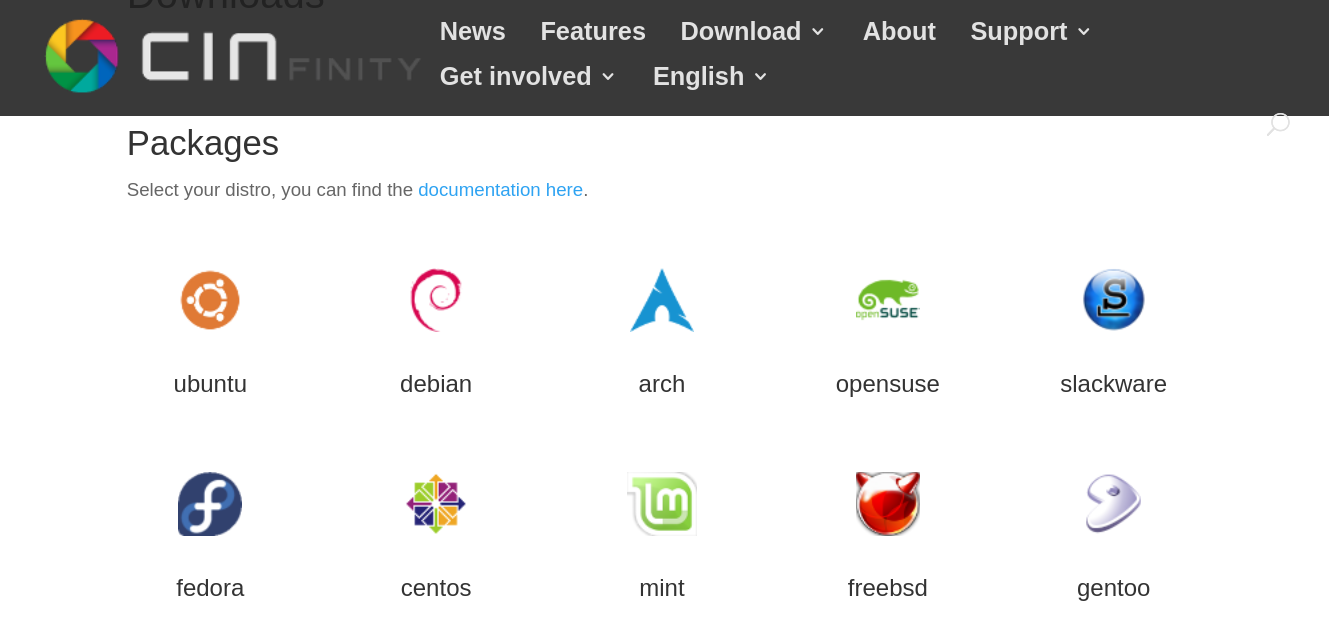
\includegraphics[width=1.0\linewidth]{download-distros.png}
    \caption{Screencast of the website Download page for installing \CGG{} for various O/S.}
    \label{fig:download-distros}
\end{figure}

If you prefer to not have to take the time to build \CGG{} Infinity yourself, there are pre-built dynamic or static binaries for various versions of Ubuntu, Mint, Suse, Fedora, Debian, Centos, Arch, and Slackware linux as well as Gentoo and FreeBSD.  
A Windows 10 version installation is described in \ref{sec:ms_windows10}.
There are also 32-bit i686 Ubuntu, Debian, and Slackware versions available.  
These are updated on a fairly regular basis as long as significant code changes have been made.  
They are in subdirectories of:

{\small \url{https://cinelerra-gg.org/download/tars}
	
	\url{https://cinelerra-gg.org/download/pkgs}}

The \textbf{tars} directory contains single-user static builds for different distros.  
This is the recommended usage of \CGG{} because all of the files will exist in a single directory.
Generally all of the necessary libraries are built into the static build, but in some cases you may
have to install another library that is being called for.  
To install the single user builds, download the designated tarball from the \texttt{./tars} subdirectory and unpack as indicated below:

\begin{lstlisting}[numbers=none]
$ cd /path
$ mkdir cin
$ cd cin
$ tar -xJf /src/path/cinelerra-5.1-*.txz    # for the *, substitute your distro tarball name
\end{lstlisting}

Do NOT download the LEAP 10-bit version unless you use h265 (it can't render 8-bit h265).

The \textbf{pkgs} directory contains the standard packaged application for various distros.  
This will install a dynamic system version for users who prefer to have the binaries in the system area and for multi-user systems.  
In addition, performing the package install checks the md5sum in the file \texttt{md5sum.txt} to ensure the channel correctly transmits the package.  
There is a {\small \href{https://cinelerra-gg.org/download/README.pkgs}{README.pkgs}} file in the \texttt{download} directory with instructions so you can \textit{ cut and paste} and avoid typos; it is also shown next.

\begin{lstlisting}[numbers=none]
Depending on the distro, use the instructions below and select the appropriate 
setup operations to install, update or remove cinelerr-gg infinity.  (02/05/2020)
To upgrade, refresh repo, then replace "install" with "update", or whatever.

Email problems to cin@lists.cinelerra-gg.org
If repository problems, usually you can manually do an install by using:
 UBUNTU, MINT, DEBIAN
  wget https://cinelerra-gg.org/download/pkgs/{substitute_name}/cin_5.1.<sub_name>.deb
  and install it manually: dpkg -i cin_5.1.{substitute_filename}.deb
 ARCH
  wget https://cinelerra-gg.org/download/pkgs/{substitute_name}/cin_5.1.<sub_name>.pkg.tar.xz
  and install it manually: pacman -U cin_5.1.{substitute_filename}.pkg.tar.xz
 FEDORA
  wget https://cinelerra-gg.org/download/pkgs/{substitute_name}/cin_5.1.<sub_name>.rpm
  and install it manually: dnf install cin_5.1.{substitute_filename}.rpm
 LEAP, SUSE
  wget https://cinelerra-gg.org/download/pkgs/{substitute_name}/cin_5.1.<sub_name>.rpm
  and install it manually: zypper install cin_5.1.{substitute_filename}.rpm
 CENTOS
  wget https://cinelerra-gg.org/download/pkgs/{substitute_name}/cin_5.1.<sub_name>.rpm
  and install it manually: yum localinstall cin_5.1.{substitute_filename}.rpm

# GENTOO - there are static and dynamic tarballs for Base Release 2.6
  https://cinelerra-gg.org/download/tars/cinelerra-5.1-gentoo-20200202.x86_64-static.txz
  https://cinelerra-gg.org/download/tars/cinelerra-5.1-gentoo-20200202.x86_64.txz
  download one of the above and then refer to README.txt

# FREEBSD - there is a tarball based on FreeBSD version 12.1 at
  https://cinelerra-gg.org/download/testing/bsdcin.tar.xz
  download the above and then refer to README.txt

# FEDORA
# Replace the XX in fedoraXX in the next line with your current O/S version number
dnf install cinelerra --nogpgcheck --repofrompath cingg,https://cinelerra-gg.org/download/pkgs/fedoraXX/
##dnf erase cinelerra

# CENTOS
# Python 2 has been updated for other distros to Python 3 so you might have to create a soft link
#   to get the correct version.  For help, send email to cin@lists.cinelerra-gg.org
# first create the file /etc/yum.repos.d/cin_gg, with the following contents:
[cin_gg]
name=cingg
baseurl=https://cinelerra-gg.org/download/pkgs/centos7
gpgcheck=0
# end of cin_gg
yum install cinelerra
##yum erase cinelerra

# UBUNTU, replace ub14 with your distro id: ub16,ub18
#  Some ubuntu apt downloads register status as working 0% constantly while running the package
#   download, like ubuntu 14.  It may take a few minutes for this step so be patient.
apt install software-properties-common apt-transport-https
apt-add-repository https://cinelerra-gg.org/download/pkgs/ub14
# UBUNTU 16/18 note - This has been known to work, but things change quickly:
# VIP - for the first install, the above line adds \CGG{} to /etc/apt/sources.list but...
# Version 16/18 of Ubuntu are more strict for licensing so you will have to edit
#  the file /etc/apt/sources.list to add [trusted=yes] after deb and before https...cin...
# For example the line should be: deb [trusted=yes] https://cinelerra-gg.org/download/pkgs/ub16 xenial main
#   Or for ub18: deb [trusted=yes] https://cinelerra-gg.org/download/pkgs/ub18 bionic main
# Also, on the install you will get an error message that you can either ignore as \CGG{}
#  will run anyway, or else (the first time only) on the commnand line keyin: 
#  echo > /etc/sysctl.d/50-cin.conf "kernel.shmmax=0x7fffffff"
apt update
apt install cin
#to update a previous install (ignore any i386 errors as only 64 bit version available):
apt update
apt upgrade cin
##apt remove cin

# MINT should use the same procedure as Ubuntu, but apt-add-repository does not seem to work,
#  so use the GUI UpdateManager as follows:
#  Administration->Software Sources->Additional Repositories->Add a new repository
#    (Note instead of Administration, some versions of Mint GUI UpdateManager might be System)
#  For Mint18,add: deb [trusted=yes] https://cinelerra-gg.org/download/pkgs/mint18 xenial main
#  For Mint19,add: deb [trusted=yes] https://cinelerra-gg.org/download/pkgs/mint19 bionic main
# IMPORTANT NOTE: if you get "malformed input" error, you will have to create a file
#    by typing the command: sudo touch /etc/apt/sources.list.d/additional-repositories.list
#    then wait 10 minutes or so and try using the Gui Update Manager again.
apt update
apt install cin
#to update a previous install
apt update
apt upgrade cin
##apt remove cin

# DEBIAN uses the same basic procedure as Ubuntu.
#  The apt-add-repository varies per system so you will have to use your best judgement
apt install software-properties-common apt-transport-https
apt-add-repository https://cinelerra-gg.org/download/pkgs/debian8
OR apt-add-repository https://cinelerra-gg.org/download/pkgs/debian9
OR apt-add-repository https://cinelerra-gg.org/download/pkgs/debian10
# VIP - for the first install, the above line adds cinelerra to /etc/apt/sources.list but...
# Debian stretch/jessie/buster are more strict for licensing so you will have to edit
#  the file /etc/apt/sources.list to add [trusted=yes] after deb and before https...cin...
# For example for debian8: deb [trusted=yes] https://cinelerra-gg.org/download/pkgs/debian8 jessie main
# For example for debian9: deb [trusted=yes] https://cinelerra-gg.org/download/pkgs/debian9 stretch main
# For example for debian10: deb [trusted=yes] https://cinelerra-gg.org/download/pkgs/debian10 buster main
apt update
apt install cin
#to update a previous install
apt update
apt upgrade cin
##apt remove cin

# SUSE/LEAP/TUMBLEWEED
# (Note: you may have to zypper libavc and libiec versions if not already installed)
# cinelerra packages are unsigned so you will have to ignore: Package is not signed!
# openSUSE LEAP 15
zypper ar -f https://cinelerra-gg.org/download/pkgs/leap15/ cingg
zypper install -r cingg cinelerra   # or cinelerra10bit for 10 bit
# openSUSE LEAP 42 
zypper ar -f https://cinelerra-gg.org/download/pkgs/leap42/ cingg
# as of 42.3 SUSE there is a new requirement, so you will need to add:
zypper mr -G cingg
zypper install -r cingg cinelerra   # or cinelerra10bit for 10 bit
# openSUSE TUMBLEWEED
zypper ar -f https://cinelerra-gg.org/download/pkgs/tweed/ cingg
# as of 42.3 SUSE there is a new requirement, so you will need to add:
zypper mr -G cingg
zypper install -r cingg cinelerra
##zypper remove cinelerra	    # or cinelerra10bit for 10 bit
#to update a previous install (assuming you enabled autorefresh as above)
zypper refresh cingg
zypper up cinelerra  # or cinelerra10bit for 10 bit

# SLACKWARE, substitute slk32 for slk64 and i486-1 for x86_64-1
wget -P /tmp https://cinelerra-gg.org/download/pkgs/slk64/cin-{date}-slk64-x86_64.txz
installpkg /tmp/cin...    # name you used in the above line
#to update a previous install
upgradepkg /tmp/cin...    # name you used in the above line
##removepkg cin

# ARCH linux
#  (A loosely defined list of packages that you should install first is listed in this file:
#   https://www.cinelerra-gg.org/download/pkgs/README.arch   )
# first edit the file /etc/pacman.conf, to include the following:
[cingg]
SigLevel = Optional TrustAll
Server = https://cinelerra-gg.org/download/pkgs/arch
# end of cingg
#
# next run from a window the following 2 commands;
pacman -Syu
pacman -S cin
# NOTE: the first line above updates your Arch system to the current rolling release and the second
#  line updates \CGG{} based on the rolling release that was in effect on the last day of the month.
#  Please complete the 2 steps above in order, one right after the other to avoid risk of a partial upgrade.
#  Due to the unpredictability of when Arch libraries are updated, performing an install of \CGG{} at
#  any time other than shortly after the last day of the month when the new build package is created,
#  could lead to library incompatibilities.  In that case, please consider using the Arch static tar file
#  for installation instead.
#to remove a previous install
##pacman -R cin
\end{lstlisting}

\section{Windows 10 with Cygwin for \CGG{} Limited}%
\label{sec:ms_windows10}

To run \CGG{} on a Windows 10 computer, you will need to have Cygwin installed on your system, 
along with the  \CGG{} static tar and a patched library: libxbc.  This setup has been tested 
with Windows 10, version 1909, on an HP EliteBook 820 at 2.3 GHz.

This limited version provides \textit{core} functionality at this time with the standard Windows FFmpeg
executable, meaning that specific modifications in FFmpeg needed for \CGG{} are not available. 
Limited capabilities include only a few render output formats available - for example \textit{mov}, \textit{qt} 
as \textit{mjpeg}, and \textit{mpeg} for videos and \textit{avi} and \textit{qt} as \textit{s16le} 
for audio, but not \textit{mkv} or \textit{mp4}.  
This is due to the fact that several codec and utility libraries are not currently compiled to 
work with Windows.

\underline{Installing Cygwin:}

Cygwin is an environment that runs natively on Windows which allows Unix programs to be compiled 
and run on Windows.  With cygwin installed on your Windows 10 computer, you will be able to run 
\CGG{}.  Before installing cygwin, you need to be warned that the Avast anti-virus software 
kills files necessary for cygwin installation and execution, so you will have to remove it and 
use alternative anti-virus software (the standard default already included with Windows 10 
is Defender). Below are the steps for installation:

\begin{enumerate}
	\item Download cygwin for your 64-bit computer at: {\small \url{https://www.cygwin.com/}}
	\item Generally just take the defaults as they show up, but the next steps show what comes up.
	\item When a warning window pops up, click \textit{Yes}.
	\item Click \textit{Next}.
	\item Choose \textit{Install from Internet} option and then click \textit{Next}.
	\item Choose your desired directory by clicking on Browse button. Choose \textit{All Users (Recommended)} and then click \textit{Next}.
	\item Choose the local package directory where you would like your installation files to be placed. Click \textit{Next}.
	\item Choose \textit{Direct Connection} if you are using Internet with plug and play device. Click \textit{Next}.
	\item Choose any download site preferably "cygwin.mirror.constant.com" and then click \textit{Next}.
	\item For list of things to install, leave all set to \textit{Default} except these to \textit{Install} instead:

\begin{tabular}{ll}
	base& devel\\
	gnome& graphics\\
	system& video\\
	X11 \\
\end{tabular}

     This install takes a long time; approximately 2 hours on an EliteBook and requires approximately 20GB storage.
	\item Finally you will want to have the icons on your desktop (already default) and then click \textit{Finish}.
\end{enumerate}

Then to install the \CGG{} tar files, you will need to start a cygwin console terminal from the startup menu as shown here:
	\texttt{Start $\rightarrow$ Cygwin $\rightarrow$ Cygwin64} Terminal

\underline{Installing \CGG{}:}

\begin{enumerate}
	\item Download the tar file at:\\
	 {\small \url{https://cinelerra-gg.org/download/testing/libxcb-bld.tar.bz2}}
	\item Install libxbc from the tar file -- installs into \texttt{/usr/local} and requires approximately 21MB storage.
\begin{lstlisting}[numbers=none]
	$ tar -C /usr/local -xJf /path/libxcb-bld.tar.bz2
\end{lstlisting}
The libxcb path repairs an error (XIOError), which stops Cinelerra.
	\item Download the tar file at:\\
	{\small \url{https://cinelerra-gg.org/download/testing/cygcin-bld.tar.bz2}}	
	\item Install cygcin from the tar file - this installs into home directory.  Note this is cygcin NOT cygwin. You must change the \texttt{path} below to the name of the path where you downloaded the tar file.
\begin{lstlisting}[numbers=none]
	$ cd
	$ tar -xJf /path/cygcin-bld.tar.bz2
\end{lstlisting}
\end{enumerate}
This creates \texttt{\~{}/cygcin} , a user build installation of \CGG{} and requires approximately 400MB storage.

\underline{Running \CGG{}:}

You will need to start a cygwin desktop from the startup menu:
\begin{enumerate}
	\item \texttt{Start$\rightarrow$ Cygwin-X $\rightarrow$ Openbox}

You should start a console controlling terminal so that you can see program logging.
	\item \texttt{Start$\rightarrow$ Cygwin $\rightarrow$ Cygwin64} Terminal

This opens a separate window that can survive a cygwin hang and bugs. Without these logs, it is much more difficult to use.

	\item Type into that console controlling window, the following:
\begin{lstlisting}[language=bash,numbers=none]
	$ export DISPLAY=:0.0
\end{lstlisting}
	\item Change directories to where \CGG{} is installed:
\begin{lstlisting}[numbers=none]
	$ cd /path/cygcin    (NOT cygwin)
\end{lstlisting}
	\item Finally keyin:
\begin{lstlisting}[numbers=none]
	$ ./cin
\end{lstlisting}
which starts up your 4 \CGG{} windows.
\end{enumerate}

The most noticeable difference from the Linux versions is that \CGG{} seems to run 
very slowly on Windows 10. You must be very tolerant and patient to see this work.  
It can however exhibit astonishing speed when encoding.  \CGG{} has to be downgraded significantly due to lack of supported interfaces, codecs (for example h264/h265), and utilities.  
The only graphics driver is X11 and the only sound driver is pulseaudio.  Almost all configurable
omissions are applied to this build.  

\underline{\CGG{} build on cygwin from source code:}

\begin{enumerate}
	\item Download and install ffmpeg into /usr/local :

   	download ffmpeg (currently 4.2.2)
\begin{lstlisting}[numbers=none]
	$ cd /tmp
	$ tar -xJf /path/ffmpeg-4.2.2.tar.bz2
	$ cd ffmpeg-4.2.2
	$ ./configure
	$ make -j
	$ make install
\end{lstlisting}
	\item Download and install a patched libxcb:
\begin{lstlisting}[numbers=none]
	$ cd /tmp
	$ rm -rf libxcb-1.13/
	$ tar -xf /path/libxcb-1.13.tar.bz2
	$ cd libxcb-1.13/
	$ patch -p1 < /path/cinelerra-5.1/thirdparty/src/libxcb.patch1
	   patching file configure.ac
	   patching file src/xcb_in.c
	$ ./autogen.sh
	$ ./configure
	$ make -j
	$ make install
\end{lstlisting}
	\item Download cinelerra-gg:
\begin{lstlisting}[numbers=none]
	$ cd /build_path/
	$ git clone "git://git.cinelerra-gg.org/goodguy/cinelerra.git"
	$ cd cinelerra-gg/cinelerra-5.1
\end{lstlisting}
	\item Apply cygwin patch:
\begin{lstlisting}[numbers=none]
	$ patch -p2 < blds/cygwin.patch
\end{lstlisting}
	\item Run the build with:
\begin{lstlisting}[numbers=none]
	$ ./blds/cygwin.bld
\end{lstlisting}
\end{enumerate}

This produces a directory: $/build\_path$/cinelerra-gg$/cinelerra$-5.1/bin \newline
which is used to create the cygcin archive.

Currently, the targets are not stripped and can be run from gdb.
There is only very limited signal handler dmp file support.
Running gdb from inside a desktop resident console (not a cygwin64 window) will hang cygwin (and cin) when it hits a breakpoint.  You must run from an external console window to avoid this issue.


\section{Distribution Systems with \CGG{} Included}%
\label{sec:distribution_systems_with_cinelerra_included}

There are also some special complete distribution systems available that include \CGG{} for audio and video production capabilities.

\textbf{AV Linux} is a downloadable/installable shared snapshot ISO image based on Debian. 
It provides the user an easy method to get an Audio and Video production workstation without the hassle of trying to find and install all of the usual components themselves. 
Of course, it includes \CGG{}!  
It is at:

\begin{center}
	{\small \url{http://www.bandshed.net/avlinux/}}
\end{center}

\textbf{Bodhi Linux} is a free and open source distribution that comes with a curated list of open source software for digital artists who work with audio, video, includes \CGG{}, games, graphics, animations, physical computing, etc.  
It is at:

\begin{center}
	{\small \url{https://gitlab.com/giuseppetorre/bodhilinuxmedia}}
\end{center}	

\section{Cinx and a “Bit” of Confusion}%
\label{sec:cinx_and_a_bit_of_confusion}

Cinx is the exact same program as Cin.  
The X (x) represents the roman numeral 10 for 10-bit as opposed to 8-bit standard.  
The third-party library used for x265 must be specially compiled with \texttt{--bit-depth=10} in order to produce 10-bit rendered output.  
This build will not be able to output 8-bit depth which means you have to retain the Cin version also.  
Whatever build ffmpeg is linked to will determine what bit depth it can output.  
This is why there have to be separate builds.  
If you install both packages, Cin and CinX, you may get \textit{file conflicts of same file name} --- just continue.

Keep in mind that the regular 8-bit version works on 8-bit bytes --- the standard word size for computers, but the 10-bit version has to use 2 words to contain all 10 bits so you can expect rendering to be as much as twice as slow.  
There is also a 12-bit version for consideration but currently the results are simply the same as 10-bit with padding to make 12-bit so it is of no value.

















